\documentclass[11pt]{article}
\usepackage{fontspec}
% \setmainfont{Times New Roman} 
\usepackage{amsmath, amssymb, hyperref}
\usepackage[a4paper, vmargin={0.45in,0.45in},hmargin={1in,1in}]{geometry}
\usepackage{enumitem}
\setlist[itemize]{noitemsep, topsep=0pt, parsep=0pt, partopsep=0pt}
\setlist[enumerate]{noitemsep, topsep=0pt, parsep=0pt, partopsep=0pt}
\usepackage{titlesec}
\usepackage{graphicx} 
\usepackage{setspace}
\usepackage{nopageno}

% \spaceskip=0pt
% \setlength{\parskip}{0pt}
% \titlespacing*{\section}{0pt}{04\baselineskip}{0.4\baselineskip}
% \titlespacing*{\subsection}{0pt}{0.3\baselineskip}{0.3\baselineskip}
% \titlespacing*{\paragraph}{0pt}{0.16\baselineskip}{0.5\baselineskip}


\begin{document}

% % 封面页
\begin{titlepage}
    \centering
    
    \vspace*{3cm}
    
    {\LARGE \textbf{IT5005 Project Final Report (Milestone 4)\\ YOLO and Tracking Algorithms}}
    
    \vspace{2cm}
    
    {\Large \textbf{Group 16}}
    
    \vspace{2cm}
    
    {\Large \textbf{Team Members:}}
    
    \vspace{1cm}
    
    \begin{tabular}{ll}
        JIANG Zhuosong & A0314591E \\
        LEE Bing Cheng & A0297134Y \\
        LI Yizhe & A0304167J \\
        LIU Yichao & A0304386A \\
        MA Kuangxuan & A0304242W
    \end{tabular}
    
    \vspace{2cm}
    
    \vspace{1cm}
    
    {\Large \today}
    
\end{titlepage}

\newpage

\makeatother
\tableofcontents
\newpage

\section{Introduction}
Object detection evolved from traditional methods to deep learning approaches, with \textbf{YOLO (You Only Look Once)} addressing speed limitations by reformulating detection as a single regression problem. YOLO achieves real-time performance while maintaining competitive accuracy by predicting bounding boxes and classes in one evaluation. When combined with tracking algorithms like \textbf{ByteTrack}, YOLO enables real-time multi-object tracking across video frames, serving applications from autonomous vehicles to surveillance systems. This combination provides temporal consistency while reducing computation, making it ideal for time-sensitive applications (Terven et al., 2023).

\section{The Evolution of YOLO Architectures}

\subsection{Early Development: YOLOv1-v3}
YOLOv1 (Redmon et al., 2016) pioneered the end-to-end approach with grid-based prediction but struggled with small objects. YOLOv2 added anchor boxes and Darknet-19 with batch normalization (Redmon \& Farhadi, 2017), while YOLOv3 incorporated Darknet-53 with residual connections for improved multi-scale detection (Redmon \& Farhadi, 2018).

\subsection{Modern Architecture: YOLOv4-v5}
YOLOv4 established the backbone-neck-head structure with CSPDarknet53 and PANet (Bochkovskiy et al., 2020). YOLOv5 reimplemented these concepts in PyTorch with SPPF and AutoAnchor, offering various model sizes for flexible deployment (Ultralytics, 2020).

\subsection{Recent Innovations: YOLOv6-v8}
YOLOv6 introduced EfficientRep backbone and decoupled detection heads (Li et al., 2022). YOLOv7 featured E-ELAN modules for optimized feature transfer and improved RepConv (Wang et al., 2022). YOLOv8, the latest version, as shown in Fig 1, implements the lighter C2f module instead of CSP blocks and adopts an anchor-free architecture with fully decoupled heads for classification, regression, and confidence estimation (Jocher et al., 2023).

\section{Architectural Components and Innovations}

\subsection{C2f Backbone Module}
YOLOv8 replaces traditional CSP blocks with the C2f module, which optimizes computational efficiency. The C2f module can be mathematically represented as:

\begin{equation}
C2f(X) = Concat[X_{first}, F_n(F_{n-1}(...F_1(X_{second})))]
\end{equation}

Where $X$ is split into $X_{first}$ and $X_{second}$ along the channel dimension, and $F_i$ represents the $i$-th convolutional block in the module. Unlike standard CSP, C2f employs dense connections where each layer receives feature maps from all preceding layers:

\begin{equation}
F_i(X) = Conv(Concat[X, F_{i-1}, F_{i-2}, ..., F_1])
\end{equation}

This formulation allows for more efficient gradient flow during backpropagation and reduces computational complexity by approximately 15\% compared to YOLOv7's backbone.

\subsection{Anchor-Free Detection Head}
YOLOv8 employs a fully anchor-free detection approach. For an input image divided into an $S \times S$ grid, each grid cell directly predicts:

\begin{equation}
\hat{y} = \{p_c, b_x, b_y, b_w, b_h, p_1, p_2, ..., p_C\}
\end{equation}

Where:
\begin{itemize}
\item $p_c$ is the confidence score
\item $(b_x, b_y)$ are the center coordinates relative to the grid cell
\item $(b_w, b_h)$ are width and height relative to the input image
\item $p_i$ is the probability of class $i$ given an object is present
\end{itemize}

Unlike anchor-based approaches, YOLOv8's bounding box parameters are predicted as direct offsets from grid cell positions rather than as offsets from predefined anchor boxes.

\subsection{Decoupled Head Architecture}
YOLOv8 implements separate branches for classification, regression, and confidence estimation:

\begin{align}
Classification: C(F) &= \sigma(W_c \cdot F + b_c) \\
Regression: R(F) &= W_r \cdot F + b_r \\
Confidence: O(F) &= \sigma(W_o \cdot F + b_o)
\end{align}

Where $F$ represents features from the neck, $W$ and $b$ are learnable parameters, and $\sigma$ is the sigmoid activation function. This decoupling allows each task to optimize independently, reducing training conflicts.

\subsection{Loss Function Formulation}
YOLOv8 employs a composite loss function:

\begin{equation}
L_{total} = \lambda_{cls}L_{cls} + \lambda_{box}L_{box} + \lambda_{dfl}L_{dfl}
\end{equation}

Where:
\begin{itemize}
\item $L_{cls}$ is the Binary Cross-Entropy (BCE) loss for classification
\item $L_{box}$ is the CIoU loss for bounding box regression
\item $L_{dfl}$ is the Distribution Focal Loss
\end{itemize}

The CIoU loss is defined as:
\begin{equation}
L_{CIoU} = 1 - IoU + \frac{\rho^2(b, b^{gt})}{c^2} + \alpha v
\end{equation}

Where $\rho$ is the Euclidean distance between box centers, $c$ is the diagonal length of the smallest enclosing box, $v$ measures aspect ratio consistency, and $\alpha$ is a trade-off parameter.

The Distribution Focal Loss (DFL) models bounding box coordinates as continuous distributions rather than point estimates:
\begin{equation}
L_{dfl} = -\sum_{i=0}^{n} y_i \log(p_i) + (1-y_i)\log(1-p_i)
\end{equation}
Where $p_i$ represents the probability that the target falls into the $i$-th bin of a discretized range, and $y_i$ is the ground truth distribution.

\subsection{Dynamic NMS Implementation}
YOLOv8 incorporates Dynamic NMS which adaptively adjusts the IoU threshold $T$ based on detection density:
\begin{equation}
T = T_{base} \cdot \exp(-\beta \cdot d)
\end{equation}
Where $d$ is the local detection density, $T_{base}$ is the base threshold, and $\beta$ is a scaling factor. This approach more effectively handles crowded scenes by allowing more detections in dense regions while maintaining strict filtering in sparse areas.

These technical innovations collectively enable YOLOv8 to achieve 53.9 AP on COCO with an inference time of 0.39 ms on modern GPUs, representing a significant advancement in the speed-accuracy trade-off for real-time object detection.

\section{Multi-Object Tracking Algorithms}

\subsection{Evolution of Tracking Algorithms}
Multi-object tracking (MOT) algorithms have evolved from simple motion-based approaches to sophisticated systems integrating detection confidence, appearance features, and motion prediction. Early algorithms like SORT (Simple Online and Realtime Tracking) relied exclusively on Kalman filtering and IoU-based matching, offering speed but suffering from frequent ID switches. DeepSORT enhanced this by incorporating appearance features through ReID networks, improving tracking persistence at the cost of computational efficiency.

\subsection{ByteTrack: Architecture and Innovations}
ByteTrack (Zhang et al., 2022) represents a paradigm shift in tracking-by-detection approaches. Unlike previous methods that discard low-confidence detections, ByteTrack's core innovation lies in its hierarchical association strategy.

\subsubsection{Dual-Threshold Association Strategy}
As shown in Fig 2, ByteTrack employs a two-stage matching process that intelligently utilizes all detection information:

\begin{enumerate}
    \item \textbf{First Association}: Matches high-confidence detections ($score > thresh_{high}$) with existing tracks using IoU similarity and Kalman filter predictions.
    \item \textbf{Second Association}: Recovers potentially valid objects from low-confidence detections ($thresh_{low} < score < thresh_{high}$) by matching them with previously unmatched tracks.
\end{enumerate}

This approach addresses a fundamental limitation in tracking systems: the trade-off between precision and recall. By intelligently utilizing low-confidence detections that would otherwise be discarded, ByteTrack significantly improves tracking performance in occlusion scenarios.

\subsubsection{Motion Prediction with Kalman Filtering}
ByteTrack employs Kalman filtering for motion prediction, mathematically expressed as:
\begin{align}
\hat{x}_t &= Fx_{t-1} + Bu_t \\
P_t &= FP_{t-1}F^T + Q
\end{align}

Where $x_t$ represents the state vector (position and velocity), $F$ is the state transition matrix, $P_t$ is the covariance matrix, and $Q$ represents process noise. This recursive estimation allows ByteTrack to predict object positions even during brief occlusions.

\subsection{ByteTrack Workflow and Advantages}

ByteTrack operates through a systematic workflow that maximizes tracking efficiency:

\begin{enumerate}
    \item \textbf{Detection}: Object detections are generated on each video frame by models such as YOLO, with each detection assigned a confidence score.
    
    \item \textbf{Confidence-Based Splitting}: Detections are categorized as high-confidence or low-confidence based on predefined thresholds.
    
    \item \textbf{Two-Stage Association}: The algorithm performs first association with high-confidence detections, followed by second association with low-confidence detections for unmatched tracks.
    
    \item \textbf{Kalman Filter Update}: Tracks are updated using the Kalman filter, predicting future states based on previous information.
    
    \item \textbf{Track Management}: Successfully updated tracks are maintained, while persistently unmatched tracks are eventually discarded.
\end{enumerate}

ByteTrack achieves state-of-the-art performance with several distinct advantages:

\begin{itemize}
    \item \textbf{Superior Performance}: Achieves 76.3 MOTA on MOT17 benchmark without requiring complex appearance features.
    
    \item \textbf{Computational Efficiency}: Maintains real-time performance by avoiding additional neural networks for appearance modeling.
    
    \item \textbf{Occlusion Handling}: Reduces track fragmentation by up to 32\% compared to SORT through its two-stage association strategy.
    
    \item \textbf{Higher Recall}: Utilization of low-confidence detections reduces the risk of object loss during tracking.
    
    \item \textbf{Reduced ID Switches}: Second-stage matching and Kalman filtering prevent frequent ID switches in cluttered environments.
    
    \item \textbf{Simplicity and Adaptability}: Easily integrates with various detection frameworks, particularly YOLO-based systems.
\end{itemize}

As shown in Table 1, ByteTrack achieves the highest performance metrics while maintaining real-time capability, making it the preferred choice for applications ranging from autonomous driving to intelligent surveillance systems. A more detailed comparison of tracking algorithms is provided in Table 2.

% \subsection{Synthesis with YOLO for Complete Detection-Tracking Pipeline}
% In the context of YOLO-based detection systems discussed in previous sections, ByteTrack forms an ideal complementary component. This synergy creates a complete detection-tracking pipeline that maximizes both accuracy and efficiency:

% \begin{itemize}
%     \item YOLO provides high-quality detections with class information and confidence scores
%     \item ByteTrack leverages these detections to maintain temporal consistency through its sophisticated association strategy
%     \item The C2f backbone module in YOLOv8 (Section 3.1) complements ByteTrack's computational efficiency
%     \item YOLO's anchor-free detection approach (Section 3.2) provides precise bounding boxes that improve ByteTrack's IoU-based matching
% \end{itemize}

% This integration creates a powerful real-time system that addresses the detection-tracking challenges outlined in the following section.


\section{Challenges and Advancements in Object Tracking}

\subsection{Integration of YOLO and Tracking Systems}
Building on our discussion of YOLO architectures and ByteTrack, their integration forms a complete Tracking-by-Detection pipeline where YOLO provides detection data and ByteTrack associates objects across frames. This synergy leverages both the computational efficiency of YOLOv8's C2f module and ByteTrack's dual-threshold association strategy.

\subsection{Technical Challenges in Multi-Object Tracking}
Several challenges affect real-time tracking performance:

\begin{itemize}
    \item \textbf{Object Scale Variation}: As objects move away from the camera, their size changes, affecting detection reliability—directly impacting YOLOv8's anchor-free detection capabilities.
    
    \item \textbf{Small Object Detection}: YOLO architectures struggle with small objects due to limited feature representation, creating a weaker training signal (Kondrackis, 2024). This challenges the multi-scale detection capabilities discussed in Section 2.
    
    \item \textbf{Occlusion Handling}: Partially visible objects cause detection inconsistencies (Han et al., 2023), though ByteTrack's second association stage helps mitigate this issue.
    
    \item \textbf{ID Switching}: Despite ByteTrack's improvements, tracking algorithms still struggle with maintaining consistent object identity during brief occlusions (Huang et al., 2024).
\end{itemize}

\subsection{Performance-Resource Trade-offs}
As demonstrated in the evolution of YOLO architectures (Section 2), improving detection often means scaling computational resources:

\begin{itemize}
    \item Larger YOLO models (YOLOv8x vs. YOLOv8n) offer better accuracy but at the cost of inference speed.
    \item This trade-off directly affects the real-time capability of the tracking system, particularly relevant to the architectural optimizations outlined in Section 3.
\end{itemize}

\subsection{Data-Centric Improvements}
Beyond algorithmic advances, dataset quality significantly impacts tracking performance (Famili et al., 1997). Well-curated training data that matches deployment conditions can substantially improve detection reliability before tracking algorithms are applied.

\subsection{Future Directions}
While this report focuses on Tracking-by-Detection with YOLO and ByteTrack, emerging end-to-end approaches like MOTRv2 (Zhang et al., 2023) are challenging the traditional paradigm. However, as evidenced by our architectural analysis, the optimal approach remains application-dependent, with speed-critical scenarios favoring the YOLO+ByteTrack combination discussed throughout this report.

\newpage
\section{Appendix: Figs \& Tables}
\begin{table}[h]
    \centering
    \begin{tabular}{|l|c|c|c|c|}
        \hline
        \textbf{Algorithm} & \textbf{MOTA} & \textbf{IDF1} & \textbf{Real-time?} & \textbf{Key Feature} \\
        \hline
        SORT & 59.8 & 53.8 & Yes & IoU + Kalman Filter \\
        DeepSORT & 61.4 & 62.2 & No & Appearance + Motion \\
        FairMOT & 73.7 & 72.3 & Yes & Joint Detection + ReID \\
        OC-SORT & 75.5 & 75.8 & Yes & Camera Motion Compensation \\
        \textbf{ByteTrack} & \textbf{76.3} & \textbf{77.3} & \textbf{Yes} & \textbf{Dual-threshold Association} \\
        \hline
    \end{tabular}
    \label{tab:mot17_results}
    \caption{Performance comparison on MOT17 benchmark}
\end{table}

\begin{table}[h]
    \centering
    \begin{tabular}{|p{1.8cm}|p{3.5cm}|p{4.1cm}|p{4.1cm}|}
        \hline
        \textbf{Algorithm} & \textbf{Key Feature} & \textbf{Strength} & \textbf{Weakness} \\
        \hline
        SORT (2016) & Kalman + Hungarian Algorithm (IoU based) & Fast, simple to implement & Prone to ID switches, no appearance modeling \\
        \hline
        DeepSORT (2017) & ReID + Motion (Kalman Filter) & Robust to occlusion, more stable ID tracking, reduces ID switches by combining motion and appearance metrics & Computationally expensive due to feature extraction \\
        \hline
        FairMOT (2020) & Joint detection + ReID & Balanced detection and tracking accuracy in crowded scenes & Complex training \\
        \hline
        ByteTrack (2021) & Hierarchical association using high/low confidence detections & Recovers occluded or low-score objects & Relies on detector quality \\
        \hline
        OC-SORT (2022) & Motion-centric updates & Handles camera motion & Requires tuning for scenes, lacks appearance modeling \\
        \hline
    \end{tabular}
\label{tab:tracking_algorithms}
\caption{Comparison of Tracking Algorithms}
\end{table}
\newpage

\begin{figure}[h]
    \centering
    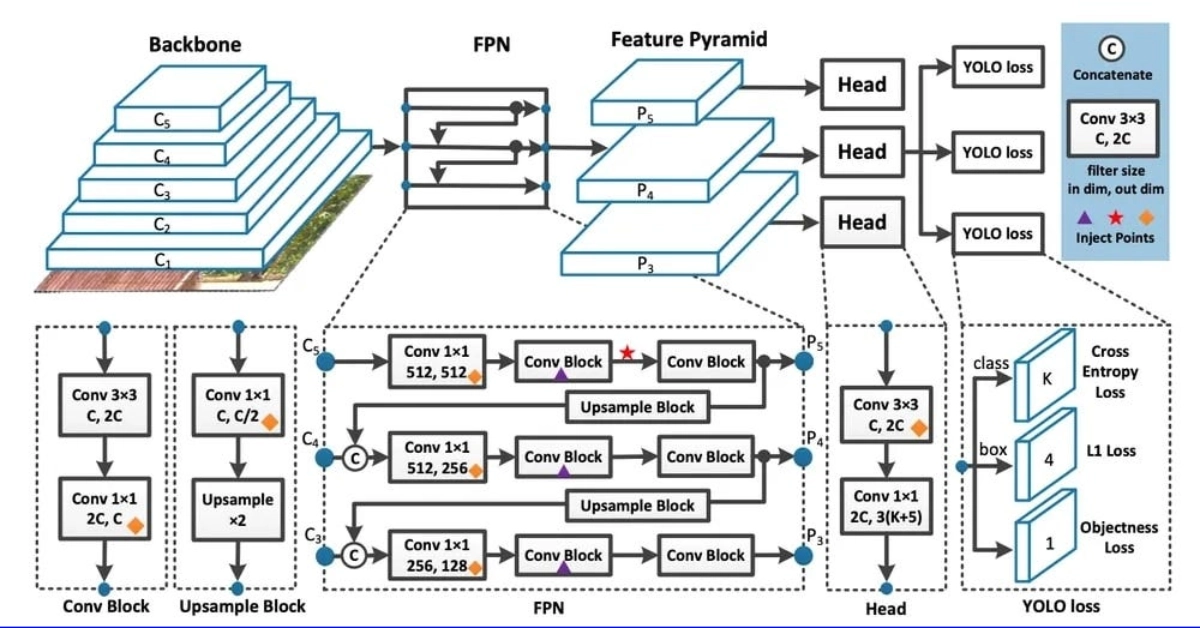
\includegraphics[width=0.8\textwidth]{figs/yolo-arch.png}
    \caption{YOLO Architecture}
    \label{fig:yolo_architecture}
\end{figure}

\begin{figure}[h]
    \centering
    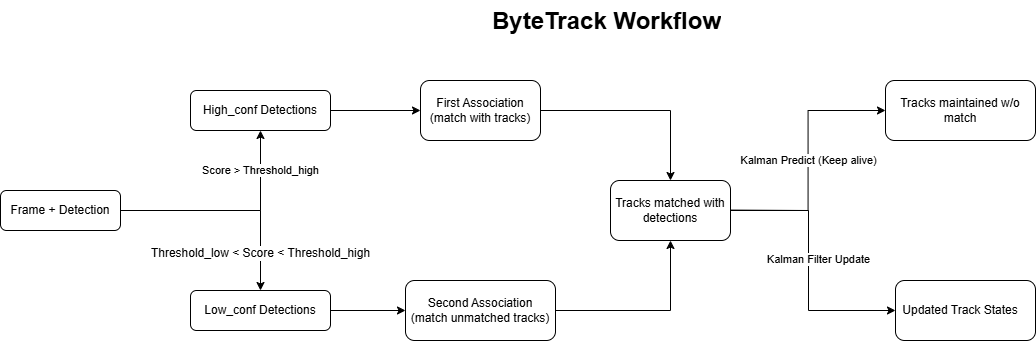
\includegraphics[width=0.8\textwidth]{figs/bytetrack-workflow.png}
    \caption{ByteTrack Workflow}
    \label{fig:byetrack_workflow}
\end{figure}


\newpage
\section{References}
\begin{itemize}
    \item Bochkovskiy, A., et al. (2020). YOLOv4. arXiv:2004.10934.
    \item Wang, C.Y., et al. (2022). YOLOv7. arXiv:2207.02696.
    \item Redmon, J., Divvala, S., Girshick, R.,\& Farhadi, A. (2016). You Only Look Once: Unified, Real-Time Object Detection. CVPR, 779–788.
    \item Szegedy, C., et al. (2015). Going Deeper with Convolutions. CVPR.
    \item Lin, M., Chen, Q.,\& Yan, S. (2013). Network in Network. arXiv:1312.4400.
    \item Terven, J.,\& Córdova-Esparza, D.-M. (2023). A Comprehensive Review of YOLO Architectures in Computer Vision: From YOLOv1 to YOLOv8 and YOLO-NAS. Machine Learning and Knowledge Extraction, 5(4), 1680–1716. https://doi.org/10.3390/make5040083
    \item Redmon, J.,\& Farhadi, A. (2017). YOLO9000: Better, Faster, Stronger. arXiv:1612.08242.
    \item Redmon, J.,\& Farhadi, A. (2018). YOLOv3: An Incremental Improvement. arXiv:1804.02767.
    \item Bochkovskiy, A., Wang, C.Y.,\& Liao, H.Y.M. (2020). YOLOv4: Optimal Speed and Accuracy of Object Detection. arXiv:2004.10934.
    \item Wang, C.Y., Bochkovskiy, A.,\& Liao, H.Y.M. (2022). YOLOv7: Trainable bag-of-freebies sets new state-of-the-art for real-time object detectors. arXiv:2207.02696.
    \item Jocher, G., et al. (2023). YOLOv8 by Ultralytics. https://github.com/ultralytics/ultralytics 
    \item Kalman, R. E. (1960). "A New Approach to Linear Filtering and Prediction Problems." ASME. J. Basic Eng. March 1960; 82(1): 35–45. https://doi.org/10.1115/1.3662552
    \item Zhang, Y., Sun, P., Jiang, Y., Yu, D., Weng, F., Yuan, Z., Luo, P., Liu, W., \& Wang, X. (2022). ByteTrack: Multi-object tracking by associating every detection box. arXiv. https://arxiv.org/abs/2110.06864
    \item Huang, C., Han, S., He, M., Zheng, W., \& Wei, Y. (2024). DeconfuseTrack: Dealing with Confusion for Multi-Object Tracking. 2022 IEEE/CVF Conference on Computer Vision and Pattern Recognition (CVPR), 35, 19290–19299. https://doi.org/10.1109/cvpr52733.2024.01825
    \item Famili, A., Shen, W., Weber, R.,\& Simoudis, E. (1997). Data preprocessing and intelligent data analysis. Intelligent Data Analysis, 1(1–4), 3–23. https://doi.org/10.1016/s1088-467x(98)00007-9
    \item Kondrackis, L. (2024, September 5). How to Detect Small Objects: a guide. Roboflow Blog. https://blog.roboflow.com/detect-small-objects/
    \item Han, S., Wang, H., Yu, E.,\& Hu, Z. (2023). ORT: Occlusion-robust for multi-object tracking. Fundamental Research. https://doi.org/10.1016/j.fmre.2023.02.003
    \item Zhang, Y., Wang, T.,\& Zhang, X. (2023). MOTRV2: Bootstrapping End-to-End Multi-Object Tracking by pretrained Object Detectors. 2022 IEEE/CVF Conference on Computer Vision and Pattern Recognition (CVPR). https://doi.org/10.1109/cvpr52729.2023.02112
\end{itemize}



\end{document}